			%%%% patron de format latex pour rfia 2000.
			%%%% sans garanties. Plaintes \`a envoyer \`a \dev\null.
			%%%% deux colonnes pas de num\'erotation et 10 points
			%%%% necessite les fichiers a4.sty french.sty et rfia2000.sty
			
%%%% Pour \LaTeXe
\documentclass[a4paper,french]{article}
\usepackage[francais]{babel}
\usepackage[utf8]{inputenc}
\usepackage{lmodern}
\usepackage[noend]{algpseudocode}
\usepackage{subcaption}
\usepackage{subfig} 
\usepackage{usual}
\usepackage{graphicx}
\usepackage[rflt]{floatflt}
\usepackage{mathrsfs}
\usepackage{multirow}
\usepackage{array}
\usepackage[rflt]{floatflt}
\usepackage{makecell}

\renewcommand\theadalign{cb}
\renewcommand\theadfont{\bfseries}
\renewcommand\theadgape{\Gape[3pt]}
\renewcommand\cellgape{\Gape[3pt]}
\pagestyle{plain}
			
\begin{document}
	\title{\Large\bf Gestion opportuniste du dialogue social}
			
			\author{\begin{tabular}[t]{c@{\extracolsep{3em}}c@{\extracolsep{3em}}c}
						%%%% pour quatre auteurs
						%%%%\author{\begin{tabular}[t]{c@{\extracolsep{4em}}c@{\extracolsep{4em}}c@{\extracolsep{4em}}c}
						%%%%pour plus d\'ebrouillez-vous !
						Lydia Ould Ouali${}^1$ &Charles Rich${}^2$& Nicolas Sabouret${}^1$\\
						\end{tabular}
						{} \\
				 \\
						${}^1$        LIMSI-CNRS \& Univ. Paris-Sud, Orsay, France \\
						${}^2$        	Worcester Polytechnic Institute, Worcester, MA, USA\\
						%Mon adresse complète \\
						%Mon adresse électronique
						}
						\maketitle
						%%%%  Pas de num\'erotation sur la page de titre
						\thispagestyle{empty}

\section{Introduction}

La modélisation d’agents conversationnels connaît un véritable essor dans différents domaines applicatifs où l'agent est muni d'un système de dialogue lui permettant de jouer différents rôles tels que  le rôle de compagnon \cite{sidner2013always} ou encore de conseiller \cite{bickmore2005s}. 

\par Les systèmes de dialogues existants peuvent être divisé en deux catégories; les systèmes de dialogue orienté tâches et les systèmes de dialogue sociaux. Les systèmes de dialogues orienté tâches sont les plus anciens, où les dialogues se centraient  exclusivement sur la collaboration avec l’utilisateur pour satisfaire des tâches communes \cite{allen1995spoken, allen1996robust}. Cependant, un certain nombre de recherches ont montré que l’aspect social ne peut être ignoré dans un dialogue, car ce dernier est social par définition \cite{markopoulos2005case}. Par ailleurs, \cite{moon1998intimate} a démontré que les utilisateurs préféraient interagir avec des agents dotés d'aptitudes sociales qui lui permettraient de construire une relation sur le long-terme avec l'utilisateur \cite{bickmore2005establishing}. Par conséquent, en plus des tâches à satisfaire, les chercheurs prennent en compte l'aspect social de la conversation dans la mise en œuvre de systèmes de dialogues. Ces derniers sont considérés comme des systèmes de dialogues sociaux.
 
\par Néanmoins, il existe encore peu de recherches qui s’intéressent a une modélisation explicite et dynamique de la relation sociale entre l’agent et l’utilisateur (c.-à.-d. qui évolue au cours de l'interaction). Les travaux existants se sont limités à une modélisation qui vise a améliorer la collaboration de l’agent et l'utilisateur sur une interaction limitée dans le temps. Dans le cadre d'une interaction sur long-terme (voir section \ref{RW}), une modélisation explicite du comportement social de l’agent doit être considérée, car cette dernière influence le dialogue directement, en terme de contenue et de stratégies mises en place par l’agent pour satisfaire ses buts \cite{bickmore2012empirical}.

\par La modélisation des comportements sociaux a été largement étudiée en psychologie sociale, plusieurs travaux ont analysés les différentes dimensions qui peuvent affecter le comportement social dans le cadre d’une interaction humain/ humains. Ces notions peuvent être adaptées et utilisées pour le cas d’une interaction humain agent.

 \par \emph{Laver}\cite{laver1981linguistic} définit le dialogue social comme un processus d'échange de préférences et d'opinions sur un sujet de conversation. Cet échange de préférences peut conduire les interlocuteurs à mener une négociation - sur leurs préférences - afin de trouver un compromis qui arrangerait les deux participants. Par exemple, deux interlocuteurs qui cherchent un restaurant où dîner à Paris. Ce type de négociation est nommé \emph{négociation coopérative}. Nous pouvons donc considérer un dialogue social comme un processus de négociation coopérative sur les préférences, où les stratégies employées par les interlocuteurs pour présenter leurs préférences sont directement affectées par leurs perceptions de la relation interpersonnelle.

\par Le but de cette thèse est d'étudier l'impact des relations interpersonnelles sur les stratégies de dialogue des interlocuteurs et spécialement dans le cadre d'une négociation coopérative. Nous présenterons d'abord dans la section \ref{RW} les recherches qui ont étudié l'évolution du comportement sociale de l'agent par rapport aux relations interpersonnelles. Ensuite, dans la section \ref{contribution} nous présenterons notre modèle dialogique préliminaire ainsi que son implémentation. Nous terminerons par les perspectives de ces travaux ainsi qu'un plan prévisionnel de la thèse.

%Plusieurs agents conversationnel intégrant une dimension sociale ou émotionnelle ont d’ores et déjà été proposés (e.g \cite{bickmore2012empirical, bickmore2005social}). nous proposons un modèle dialogique capable d'adapter les stratégies de dialogues de l'agent par rapport à sa perception de la relation interpersonnelle. 
\section{État de l'art}
\label{RW}
Cette section sera dédié à l'état de l'art existant autour de notre thématique de thèse. nous présenterons les systèmes de dialogues qui s'intéressent à la modélisation des relations avec l'utilisateur, ainsi qu'une représentation des relations interpersonnelles.  

\subsection{Le dialogue social}
\par Le dialogue social consiste en une conversation où les buts interpersonnels sont mis en avant et les buts orienté tâches, s'ils existent, sont mis en arrière plan \cite{bickmore2005social}. Par exemple, une personne peut avoir l'intention d'impressionner son amie et va donc initier un dialogue avec un but  tâche de trouver un restaurant où elle aimerait dîner. Comme présenté précédemment, durant cette conversation, les interlocuteurs évoqueront leurs préférences et peuvent même négocier de manière coopérative afin de trouver un terrain d'entente (par exemple, un choix de restaurant).  
%Par ailleurs, \cite{laver1981linguistic} affirme que les comportements familiers apparaissent durant des conversations entre deux personnes qui ne se connaissent pas ou qui ne sont pas familiers. 

%Durant cet échange,les interlocuteurs parlent soit de sujets neutres ou partagent des expériences personnelles, des préférences ou des opinions. Par conséquent, l'échange de préférence ou opinions peut mener les interlocuteurs à une négociation coopérative sur le sujet de conversation.


\par Il existe déjà  des travaux qui se sont intéressés à la négociation  dans le dialogue. Par exemple \cite{amgoud2000arguments, daskalopulu1998handling} qui ont mis en œuvre des modèles formels de dialogue où les agents sont capables de négocier et même d'argumenter sur leurs choix de préférences. Cependant, ces travaux ont négligé à l'aspect social du dialogue. Or,il a été prouvé que les relations sociales affectent directement le comportement des interlocuteurs \cite{bickmore2000weather, bickmore2005establishing, moon1998intimate, nass2000does} et par conséquent leurs stratégies dans le dialogue. Par exemple, une personne dominante exprime facilement ses préférences et argumente contrairement a une personne soumise. 

%\par Dans le reste de cette section, nous présenterons l'état des recherches dans le domaine du dialogue social avec un agent.

\subsection{ACA sociaux}

\par Il existe dans la littérature des  ACA sociaux  qui arrivent à modéliser leurs relations avec l'utilisateur et la gérer afin d'adapter leur comportements dans la conversation.

\par \textbf{Autom :} Le robot Autom \cite{kidd2005sociable} est conçu pour jouer le rôle d'un conseiller de perte de poids, placé dans les maisons des utilisateurs pour une intervention sur le long terme. Le robot s'intéresse principalement à trois facteurs de relations avec l'utilisateur, à savoir \textit{l'engagement, la confiance et la motivation}.  Le modèle de relation utilisé est construis sur trois étapes. La première étape est la prise de connaissance où le robot doit  d'abord encourager l'utilisateur à s'engager dans une interaction avec le système, pour ensuite le motiver à réaliser les tâches.
La seconde étape est la construction des relations avec l'utilisateur. En effet, le robot doit être explicite sur les avantages qu'il peut apporter à l'utilisateur, sa compréhension du système est obligatoire afin que l'utilisateur puisse construire une relation de confiance avec le robot qui permettra à ce dernier de répondre aux attentes de l'utilisateur.  La dernière étape est la maintenance de la relation qui est la partie la plus importante, où le robot doit s'assurer de maintient de l'engagement de l'utilisateur pour établir une relation de confiance au fil des interactions. Le système un nombre limité d'acte de langage afin d'établir et maintenir sa relation avec l'utilisateur.


\par \textbf{FitTrack: } est un des premiers systèmes à mener une étude longitudinale sur l'engagement entre l'utilisateur et un agent virtuel \cite{bickmore2005s}. Le cadre de l'étude est de changer les comportements de santé. L'agent joue le rôle d'un conseillé d'exercices avec qui les utilisateurs interagissent quotidiennement durant un mois. L'agent utilise un large éventail de techniques tirées de la psychologie sociale des relations, dont les communication personnelles méta-relationnelles, l'empathie, le dialogue social afin de construire un terrain d'entente, ainsi que la prise en compte des comportements non verbaux. Tous ces comportements sociaux ont pour but d’accroître le lien social avec l'utilisateur au cours du mois d'intervention.

\par Cependant, les comportements sociaux ne sont pas généré dynamiquement. Ils sont préalablement codé dans le dialogue de l'agent qui basé sur machine d'états fini et apparaissent selon un calendrier pré-défini (par exemple, le nombre d'interactions sociales par jour). Ainsi, le modèle relationnel évolue implicitement dans le temps (nombre d'interactions avec l'utilisateur).


\par \textbf{REA : } REA \cite{bickmore2005establishing} est un agent conversationnel incarné grandeur nature qui joue le rôle d'un agent immobilier. Le planificateur décide dynamiquement  de choisir entre le dialogue social  ou sur des un dialogue orienté tâches (poser des questions sur les besoins de logement de l'utilisateur). Un des facteurs de choix de dialogue est basé sur une évaluation de la relation actuelle avec l'utilisateur. La relation a été modélisé en utilisant un modèle tridimensionnel \cite{svennevig2000getting}, où la solidarité et la familiarité sont représentés comme des scalaires. Une dimension de confiance a été ajoutée au système pour améliore les performances de REA. La  mise à jour des  relations est basée sur le nombre et le contenu des mouvements de conversation.

\par Notre travail s'inscrit dans la continuité de ces travaux dans le sens où nous modélisons un agent conversationnel qui puisse percevoir sa relation avec l'utilisateur et adapter ses stratégies de négociation et de dialogue en fonction de cette relation. 

\subsection{Les relations interpersonnelles}
\par Les relations sociales et leurs effets sur le comportement sont au cœur de la science sociale. Il a été prouvé que la compréhension de la relation interpersonnelle est crucial pour la cognition sociale \cite{reis2000relationship}. Les recherches qui se sont intéressées à l'analyse conceptuelle des relations interpersonnelles affirment que l'essence d'une relation apparaît dans la nature de l'interaction qui se produit entre les partenaires. En outre, la relation sociale est un système dynamique qui peut se développer et continuellement changer avec les interactions \cite {reis2000relationship,svennevig2000getting}.
\par La communication entre les partenaires se développera par étapes; commençant par une interaction initiale où les partenaires partagent des informations superficielle et évoluant à une relation plus profonde où les partenaires peuvent partager plus de renseignements personnels. Par conséquent, la relation sociale de partenaires affecte directement le comportement des partenaire et leur stratégie de dialogue et donc le contenue du dialogue.


\subsubsection{Dimensions des relations interpersonnelles}
La représentation dimensionnelle des relations est la représentation la plus courante dans la littérature qui consiste à représenter les relations dans un cercle de dimensions \emph{(c.f modèles de Wiggins)}. Par conséquent, toute relation peut être située et évaluée dans cet espace dimensionnel \textit{continu}. Un des modèles les plus connus est celui de Svennevig \cite{svennevig2000getting} qui divise les relations interpersonnelles sur quatre dimensions. 
\par \textbf{Dominance:} Des chercheurs de différents domaines s'accordent pour définir la dominance ou le pouvoir comme la capacité d'influencer le comportement d'autrui. Le pouvoir peut être latent \cite{komter1989hidden} ce qui est en contradiction avec la définition d'une position dominante qui est inévitablement manifeste \cite{dunbar2005perceptions}. La dominance est une variable asymétrique dans lequel l'assertion de dominance manifestée chez un interlocuteur est satisfaite par l'acquiescement de l'autre \cite{rogers1979domineeringness}.

\par \textbf{Familiarité:} Dans le modèle relationnel de Svennevig, la définition de familiarité est basée sur la théorie de la pénétration sociale, qui décrit les étapes de l'évolution des relations à travers l'échange mutuel d'informations à la fois en profondeur (information superficielle à l'information personnelle et intime) et en largeur (de sujets étroits à un large éventail de sujets personnels).

\par \textbf{Affect:} Cette dimension représente le degré de d'appréciation qu'a chaque interlocuteur pour l'autre. Cette dimension permet aux interlocuteurs de créer l'attachement personnel afin d'améliorer la relation entre les interlocuteurs\cite{nicholson2001role}.
	
\par \textbf{Solidarité:} La dimension de la solidarité est une dimension symétrique où deux individus partagent les mêmes obligations et les droits. Elle est identifiée comme une  relation  \emph{‘vision semblable’} où les interlocuteurs ont les mêmes comportements et partagent par exemple les mêmes préférences

\par Dans le cadre de cette thèse, nous avons décider de commencer la conception de notre modèle avec la relation de dominance, car durant la collecte de données que nous avons effectué (voir section \ref{contribution}), nous avons remarqué que la relation de dominance permettait l'apparition de comportements qui nous semblent intéressants à reproduire dans un agent conversationnel.  



\section{Contribution}
\label{contribution}

\par Afin de réaliser nos objectifs, nous avons d'abord enregistré des dialogues entre deux personnes afin d'observer leurs comportements dans un cadre de dialogue social. 
Pour extraire et analyser ces comportements, nous avons annotés et analysé les dialogues  en se basant sur les travaux de Sidner \& Grosz \cite{grosz1986attention}.
 \par L'analyse menée nous a permis de détecter et et de différencier les comportements communs de ceux liés aux relations interpersonnelles. Nous avons ensuite reproduit dans des jeux de dialogues dans le modèle D4G utilisé au sein de la plate-forme de dialogue Disco que nous utilisons dans nos travaux \cite{rich2009building}. 

\par Les informations collectées grâce l'observation des comportements humains nous a guidés dans la conception de notre modèle dialogique avec une modèle mental de l'environnement de l'agent, et un modèle lui permettant de mener une négociation coopérative. 
En parallèle, nous avons modélisé un module de communication comportant cinq actes dialogiques qui lui permettent de dialoguer et négocier durant de le dialogue. 
\par Nous présenterons dans cette partie nos travaux menés. En premier temps, nous présenterons plus en détails la collecte de données et son analyse. 
	Nous présenterons ensuite notre modèle dialogique et ses différents modules ainsi que son implémentation sur Disco. 

\subsection{Collecte de données}

%Explication du procédé (image sur le coté)

Afin d'étudier la structure des dialogues enregistrés, nous nous sommes basés sur les travaux de Sidner \& Grosz \cite{grosz1986attention}  qui définit la structure du dialogue en trois composantes interdépendantes, à savoir la structure linguistique, la structure intentionnelle et la structure attentionnelle. L'analyse que nous avons effectués s'est cependant limitée à l'analyse linguistique et intentionnelle que nous présentons ci-dessous. 

\subsubsection{La structure linguistique} la structure linguistique définit le dialogue comme un ensemble séquences d'actes de dialogues. Ces actes de dialogues sont agrégées en \textbf{segments de discours (SD)} (Discourse Segments), comme des mots agrégés pour composer une phrase. De plus, tous les SD exercent certaines fonctions sur le dialogue et forment des relations entres eux.  
\par La principale difficulté rencontrée lors de la définition de la structure linguistique réside dans la définition des délimitations entre segments de discours. Une des solutions principales est d'utiliser des expressions linguistiques comme indicateurs de délimitations de SD, par exemple: premièrement, d'ailleurs... 
\par Par ailleurs, des inducteurs plus subtiles tels que l'intonation ou des changements de temps et l'aspect, sont inclus comme des délimiteurs de SD. Le terme \textbf{"cue phrases"} est défini dans ce travail pour englober la notion de délimiteur de SD. 

\textbf{Exemple} cet exemple représenté dans la \fig{ling} illustre un extrait de segmentation de dialogue réalisé sur un des enregistrements

\begin{figure}
	\fbox{	\centerline{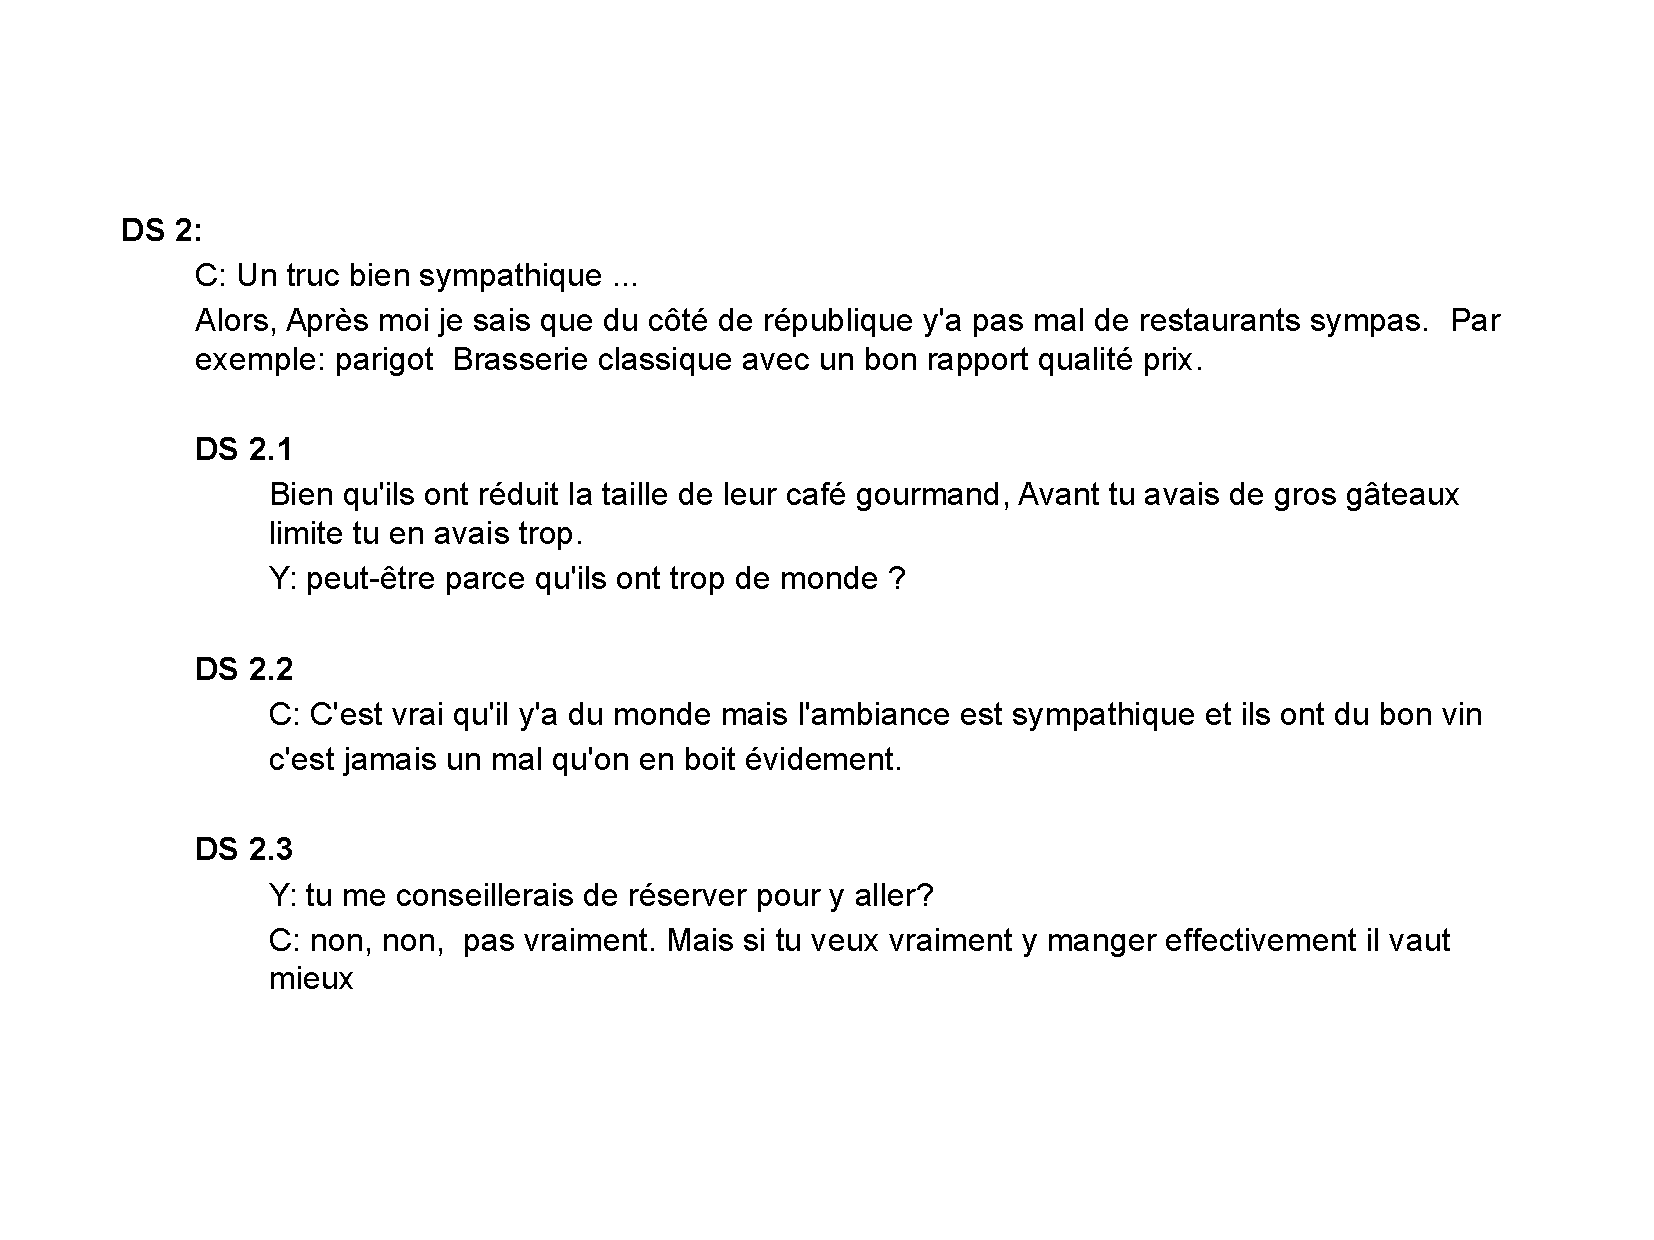
\includegraphics [width=4in]{figs/ds.pdf}}}
	\vskip 8pt
	\defig{ling}{Architecture du modèle de dialogue.}
\end{figure}

\subsubsection{La structure intentionnelle} 
Les interlocuteurs peuvent avoir plus d'une raison pour participer à une conversation. Sidner \& Grozs distinguent premièrement, le but fondamental du dialogue noté (discourse purpose \textbf{DP}) qui représente le but principal qui amène les interlocuteurs a engager un dialogue. Deuxièmement, pour chaque segment de discours on peut isoler un seul but noté (\textbf{DSP} Discourse segment purpose). Ce dernier, spécifie la contribution du segment dans la satisfaction du DP globale du dialogue. De plus, les auteurs identifient deux types de relations entres les DSPs à savoir la \textbf{dominance} et \textbf{priorité de satisfaction}. Un segment qui satisfait une intention qu'on note DSP1 peut participer à la satisfaction d'une autre qu'on nommera DSP2. Dans ce cas, on notera que DSP1 \textit{contribue à} la satisfaction de DSP2. Inversement, on note DSP2 \textit{domine} DSP1. La relation de dominance est référencé à la dominance hiérarchique des DSP.

\par \textbf{Exemple}: L'analyse intentionnelle de SDs dans la \fig{ling} nous a révélé la structure de la tâche ``Choisir un restaurant" comme illustré dans \fig{intention}.

\begin{figure}
	\fbox{	\centerline{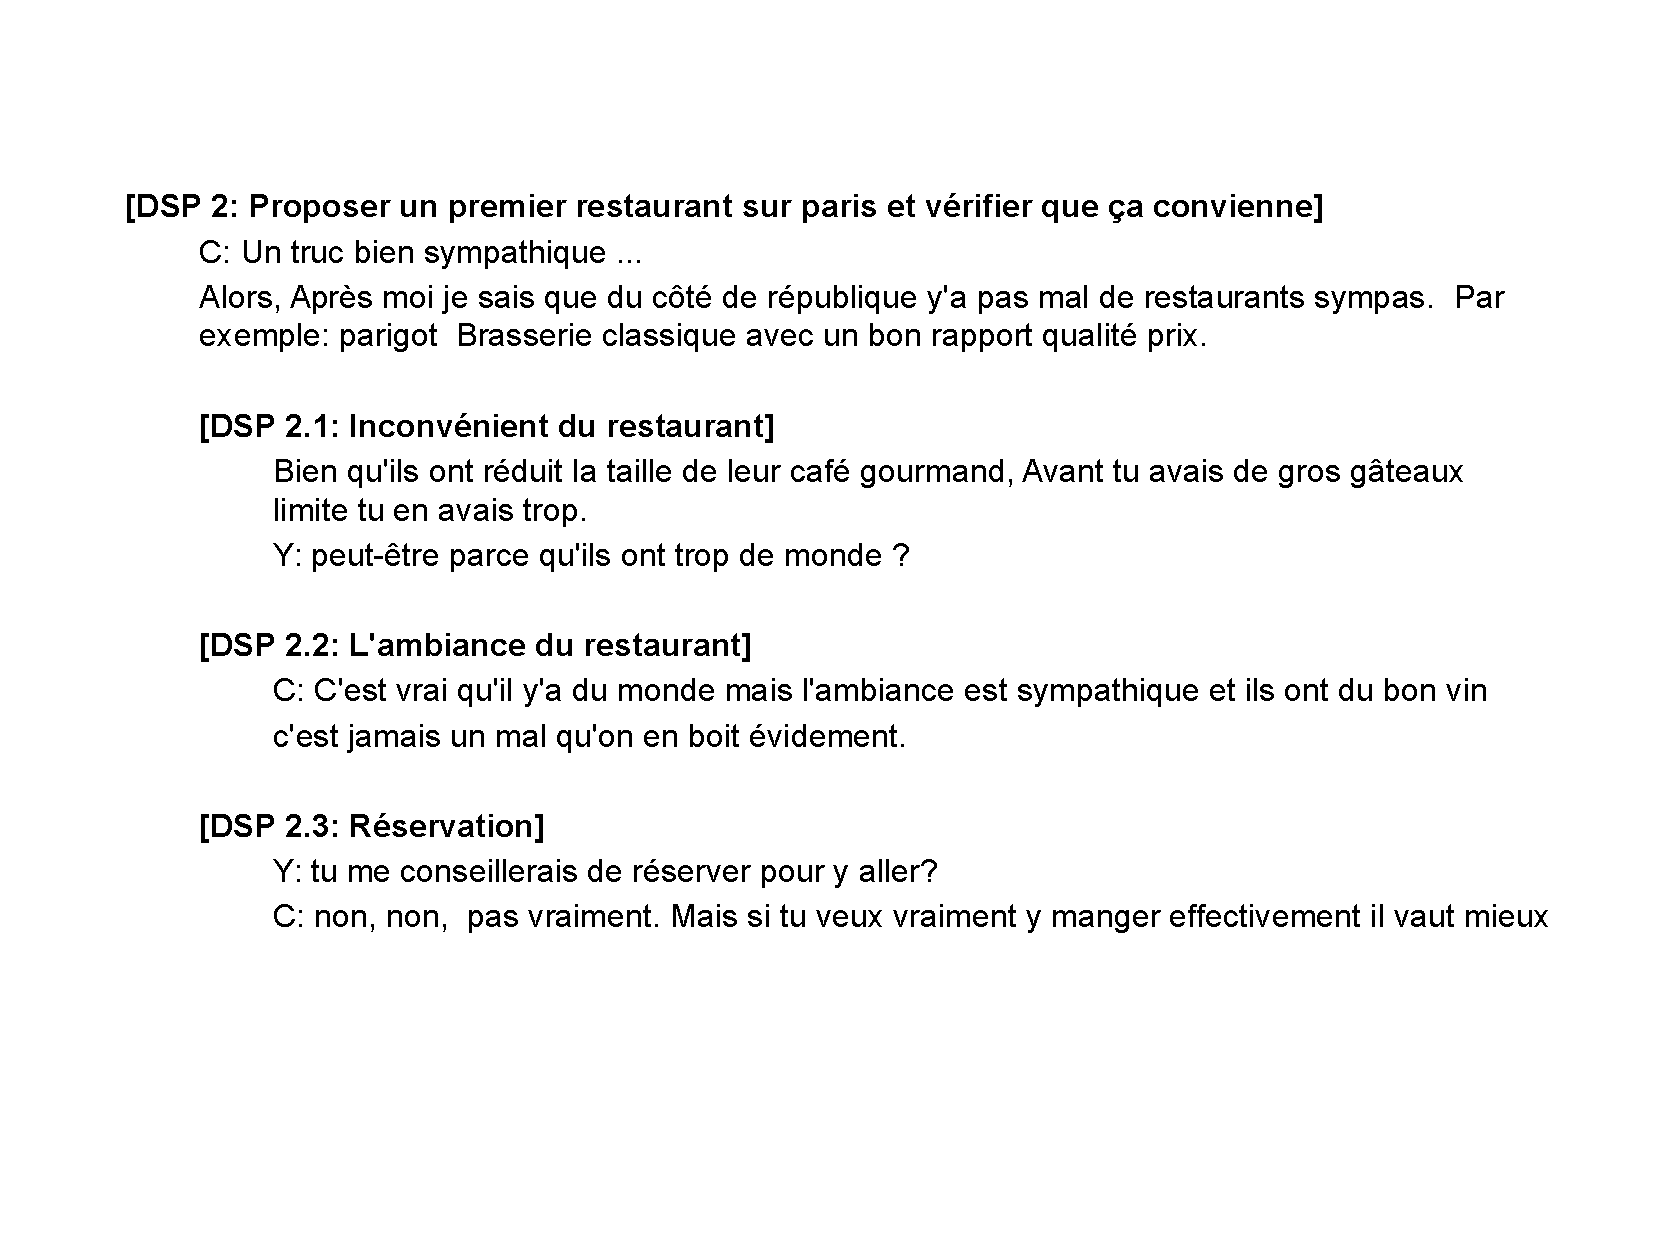
\includegraphics [width=4in]{figs/dsp.pdf}}}
	\vskip 8pt
	\defig{intention}{Architecture du modèle de dialogue.}
\end{figure}


\par Un interlocuteur qui initie un dialogue peut avoir plusieurs intentions. Il est donc important de pouvoir distinguer les différents types d'intentions. Les intentions communicatives sont destinées à être reconnues. Par exemple, l'intention de complimenter l'autre n'est satisfaite que si elle est reconnue par l'autre interlocuteur. D'autres intentions sont au contraires privées et peuvent être la motivation première pour d'un interlocuteur pour initier un dialogue. Par exemple, un interlocuteur dont le but est d'impressionner l'autre et donc l'inviter au restaurant, dans ce cas l'initiateur ne veut pas que l'autre soit au courant de ses intentions (impressionner). Par conséquent, l'intention d'initier un dialogue peut être privée. En revanche, les DSPs sont communicatifs pas exemple inviter au restaurant. 

\subsubsection{Résultats obtenus:}
\par A l'origine, la collecte de donnée a été mené dans le but d'observer des interlocuteurs menant un dialogue social. Néanmoins, l'analyse des dialogues nous a livrés des résultats intéressants qui ont pu être exploité dans la mise en œuvre de notre modèle dialogique.  Ces résultats sont expliqués dessous.

\begin{itemize}

		\item  La segmentation du dialogue en SD nous a permis d'extraire le processus que suivaient les interlocuteurs dans l'exécution de la tâche  ``trouver un restaurant''. En effet, les interlocuteurs abordait systématiquement le type de la cuisine, l'ambiance, le prix, et la localisation. 
		
		\item L'analyse intentionnelle nous a permis d'identifier les buts communicatifs et buts internes des interlocuteurs,qui nous ont guidé dans l'identification des comportements qui sont soit liées aux relations interpersonnelles ou simplement en rapport avec le sujet de conversation. Par exemple, détecter un comportement dominant dans le nombre de fois où il initie un nouvel sujet, le nombre de prise de paroles, la fréquence de propositions, l'argumentation ... ), qui nous a permis d'analyser l'évolution de la relation de dominance dans ces dialogues. 
		\item Identification d'actes de langage récurrents dans les dialogues qui nous a par la suite aidé dans la définition d'acte de dialogue pour notre agent.	
		\item Les actes de langages retrouvés dans le dialogue portent tous sur l'expression des préférences qui soutient l'idée de la négociation coopérative.
	
\end{itemize}

\par Cette analyse nous a aidé a mieux cibler notre contribution, à savoir étudier l'impact des relations dans les stratégies de dialogue.

	
	
\subsection{Modèle formel du dialogue}
\par Le modèle proposé vise à doter l'agent de connaissances qui lui permettent de mener une négociation coopérative sur un sujet de conversation sociale. L'architecture de notre modèle illustré dans la \fig{modele} se compose de trois principaux modules: un \textit{état mental} regroupant les préférences de l'agent et de l'utilisateur, un \textit{module de communication} comprenant les actes de langages que l'agent est apte à utiliser et enfin un module qui sauvegarde le \textit{contexte du dialogue} à savoir l'historique des informations échangées durant le dialogue. Nous présentons dans cette section chaque module.

\begin{figure}
	\fbox{	\centerline{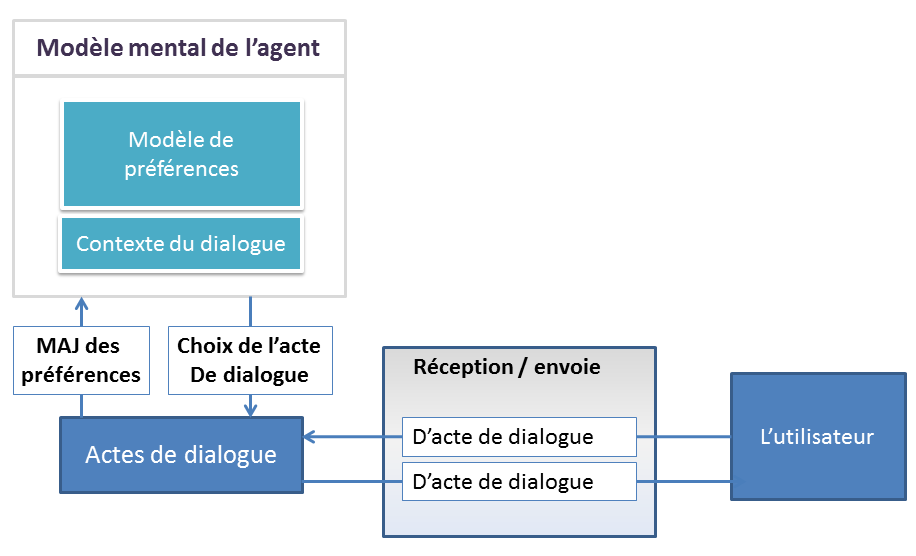
\includegraphics [width=4in]{figs/modele}}}
	\vskip 8pt
	\defig{modele}{Architecture du modèle de dialogue.}
\end{figure}

\subsubsection{L'état mental}
\par La représentation actuelle de notre modèle vise a représenter une négociation coopérative entre l'agent et l'utilisateur. Afin de mener a bien la négociation, l'agent requiert une modélisation formelle de son environnement, à savoir ses préférences, ainsi que les préférences de l'utilisateur. Nous notons donc
 \begin{itemize}
 	\item  $\mathcal{P}_{self}$ le modèle de préférences de l'agent.
 	\item $\mathcal{P}_{other}$ le modèle de préférences de l'utilisateur que l'agent aura acquis durant le dialogue.
 	\item De plus; l'agent conserve les information qu'il communique à l'utilisateur (un module de la théorie d'esprit) qu'on note $\mathcal{P}_{other-about-self}$.
 \end{itemize}

 \par Dans ce qui suit, nous présenterons le modèle formelle de préférences utilisé pour la représentation de l'état mental de l'agent.
\\

\par \textbf{Le modèle de préférence :}
Le but principal de la négociation est de choisir une \emph{option} parmi un ensemble d'options qu'inclut le thème de la négociation (et donc de la conversation). Par exemple, pour une négociation sur le thème des ``Restaurants'', l'ensemble des options à choisir peut être : ``Chuck's cake'', ``The ducking Duck'', ``Ginza sushis''\ldots \\ On note donc $\mathcal{O}$, l'ensemble des options définis pour un thème de négociation. \par Afin de pouvoir  comparer ces options, les interlocuteurs se basent sur un ensemble de critères qui reflètent les caractéristiques de ces options. Par exemples, les critères de choix d'un restaurant sont \{la cuisine, le prix, l'ambiance, la localisation\}.  On note $\mathcal{C}$ les critères des options définis dans $\mathcal{O}$. Par ailleurs, chaque critère doit être mesurable de manière a pouvoir évaluer une option même qualitativement. Donc, $\forall$ \emph{c $\in\mathcal{ C}$},  on note \emph{D$_c$} son domaine de valeurs. par exemple, le domaine de valeurs du critère de la cuisine est noté $\emph{D}_{cuisine} = \{Chinois, Italien, Indien...\}$.

\par Chaque option $O\in \mathcal{O}$ définit une valeur pour chaque critère : 
$O = \{c_1=v_1,..., c_n=v_n\}$ avec $c_i \in \mathcal{C}, \forall i \in [1,n]$ et $v_i\in \emph{D}_{c_i}$. 
Par conséquent, on note $\{v(c,O) \in \emph{D}_{c} / \forall O \in \mathcal{O}, \forall c \in \mathcal{C}\}$ la valeur \emph{objective} du critère $c$ attribué à l'option $O$. La valeur objective d'un critère est indépendante des préférences; les interlocuteurs affectent les mêmes valeurs au critères d'une option indépendamment de leurs préférences. 
Par exemple, Ginza est un restaurant japonais coûteux : $v(prix, Ginza) = couteux $ et $(cuisine, Ginza) = japonais$. 

\par Nous présentons dans ce qui suit la représentation des préférences de l'agent qui lui permet d'exprimer et décider de ses préférences.
\\ \par \textbf{Représentation des préférences :}
Nous définissons une préférence \emph{P} comme une relation transitive et antisymétrique  définit sur un ensembles d'éléments \emph{A}, tel que:

\[ \left \{
\begin{array}{l}
\emph{P(a,b)} $ : \emph{a}  est préféré à $\emph{b}. \emph{ a,b} \in \emph{A}\\
\emph{P(b,a)} $:  \emph{b} est préféré à  $\emph{a}. \emph{ a,b} \in \emph{A}\\
$Sinon, aucune . $\\
\end{array}
\right .\]

Par exemple $P_{cuisine} (Japonais, Italien)$ signifie que l'interlocuteur préfère la cuisine japonaise à l'italienne. 

\par Nous définissons des variantes pour la notion de préférences:
\begin{itemize}
	\item  \emph{P(a,*)}  = \{$\forall$ \emph{x}$\in$\emph{A}, \emph{P(a,x)}\}, représente le fait que  \emph{a} est l'élément  \textit{le plus préféré} dans \emph{A}.
	\item Par opposition, \emph{P(*,b)} = \{$\forall$ \emph{x}$\in$\emph{A}, \emph{P(x,b)}\} signifie que \emph{b} est l'élément \textit{le moins préféré} dans l'ensemble \emph{A}. 
\end{itemize}


\par Notre but est de définir des préférences sur les options de la négociation.  Nous retrouvons dans la littérature plusieurs méthodes de calcul des préférences d'une option \cite{dodgson2009multi}. Ces méthodes nommées décision multi-critères calculent les préférences d'une option selon les performances de cette dernière sur l'ensemble des critères qui la définissent. Dans l'ensemble\cite{dodgson2009multi}, le calcul des préférences d'une option est fait par inférence à partir des préférences enregistrées sur les valeurs de ses critères. Cette inférence peut être réalisée grâce à différentes méthodes comme la fonction de somme pondérée \cite{yager2012ordered} ou encore les intégrales de Choquet \cite{chouquet1953}. \\

\par  \textbf{Sélection basée sur les préférences :} Une fois que le modèle de préférences est définit avec les relations de préférences sur les valeurs des critères, l'agent dispose d'information suffisantes pour pouvoir comparer deux options et calculer la relation 
$P(O_1, O_2) / O_1, O_2 \in \mathcal{O} $.

La relation de préférence entre deux options est effectuée en calculant l'utilité de chaque option grâce a une fonction de décision multi-critères. 
Nous avons sélectionné pour notre modèle la fonction de somme pondérée \cite{yager2012ordered} qui offre une méthode d'agréger les préférences sur les valeurs des critères calculé individuellement afin d'obtenir un score d'utilité globale pour l'option.
 
\par On note  $score(a)$ le nombre des successeurs de  $a$  dans le modèle de préférence $\mathcal{P}$, ce qui signifie que $|\{x \in \mathcal{D} / (a,x) \in \mathcal{P}\}|$. 
$rang(a)$ est le score normalisé $a$, qui est calculé en triant les valeurs d'un domaine $\mathcal{D}$ par ordre croissant de leurs scores. 


Par conséquent, calculer l'utilité d'une option grace à la fonction de somme pondéré est effectué comme suit:

\[U(O) = \sum_{c_j \in \mathcal{C}}  rang_R(c_j) \times score\left( v(O, c_j) \right) \] 


\par La relation de préférence entre deux options est donc calculée en comparant leurs utilités. 
\[ P(O_1, O_2)  = \left \{
\begin{array}{l}
P(O_1, O_2)$ \textit{if}  $U(O_1) > U(O_2) \\
P(O_2, O_1)$  \textit{if}  $U(O_2) > U(O_1) \\
$  \textit{aucune n'est préférée}  $U(O_2) = U(O_1)\\
\end{array}
\right .\]

 \par \textbf{Exemple de décision}

On suppose que l'agent cherche à calculer la relation de préférence suivante:  P(Clementine, Mogoroko), tel que 
\{Mogoroko, Clementine\} $\in$ Restaurant. La description des restaurants: 
\begin{itemize}
	\item Clementine=(Cuisine =\textit{Français}, Cost=\textit{Couteux}, Location=\textit{Paris02},
	\\Ambiance=\textit{Calme}).
	\item Mogoroko=(Cuisine=\textit{Japonais}, Cost=\textit{Abordable}, Location=\textit{Paris09}, 
	\\Ambiance=\textit{Calme}).
\end{itemize}

L'utilité de chaque option est calculée comme suit:
\begin{itemize}
	\item U(Clementine)=$rang$(Cuisine)$\times score$(\textit{Français})+$rang$(Prix)$\times score$(\textit{Couteux})\\+$rang$(Localisation)$\times score$(\textit{Paris02})
	+$rang$(Ambiance)$\times score$(\textit{Calme}).
	\item U (Mogoroko)= $rang$(Cuisine)$\times score$\textit{Japonais}+$rang$(Prix)$\times score$(\textit{Abordable})\\+$rang$(Localisation)$\times score$(\textit{Paris09}) +  
	$rang$(Ambiance)$\times score$(\textit{Calme})..
\end{itemize}
Le résultat du calcul des utilités: U(Clementine)=-3 and U(Mogoroko)=5.
\\  On conclut donc que $P(Mogoroko, Clementine)$ est vraie.
(i.e Mogoroko est préféré à Clementine).

\subsubsection{Contexte du dialogue}
\par Durant le dialogue, les deux interlocuteurs échangent des informations sur leurs préférences et suggèrent des propositions pour le choix d'une option. par exemple, je préfère manger Indien ce soir, ou allons au restaurant Ginza ...

Afin de capturer ces informations, nous définissons les éléments suivants:
\begin{itemize}
	\item Une proposition est définie comme un tuple $Proposal(Type, Valeur)$ où $Type$ est soit le thème de négociation par exemple ''Restaurant``, soit un critère $c \in \mathcal{C}$ et $Valeur$:
		\subitem -  une option $O \in \mathcal{O}$ si $Type \in Topic$ 
		\subitem - une valeur de critère $v \in \emph{D}_c$ si $Type \in \mathcal{C}$
	\item Afin de garder trace de toutes les propositions soumises durant le dialogue, nous définissons ces structures de données qui stockent une proposition a chaque cycle de vie. 
		\subitem - $ Proposed$ est la liste de toutes les propositions ouvertes dans le dialogue.
		\subitem - $ Rejected$  est la liste des propositions rejetées.
		\subitem - $ Accepted$  est la liste des propositions acceptées. Il est a noté qu'il suffit qu'une option soit acceptée pour pouvoir clore la négociation. 
\end{itemize}
\subsubsection{Sémantique des actes de dialogue}
\par Les agents communiquent en utilisant des actes de dialogues qui encapsulent le message. Dans les dialogue, les messages sont considérés comme des actions. Ils sont donc définis avec des préconditions et des effets qui mettent à jours l'état mental de l'agent. Il est à noter que les préconditions sont toutes optionnelles, car le choix d'un message dépend en premier lieu de la stratégie de l'interlocuteur. Pour l'instant, les effets d'un message concernent exclusivement la mise à jour de connaissances de l'agent sur son environnement (les préférences de l'utilisateur, et les connaissances de l'utilisateur sur les préférences de l'agent). De plus, l'effet d'un message ne change en aucun cas les préférences de l'agent. 

\begin{table}
	
	\caption{\label{tab: utt} Sémantique des actes de dialogue}
	\begin{tabular}[t] {|m{0.40cm}|m{4cm}|m{2cm}|m{2.5cm}|m{3cm}|m{2.5cm}|}
		
		\hline 
		N & \thead{Utterance} & \multicolumn{2}{c|} {\thead{Preconditions}  } &  \multicolumn{2}{c|} {\thead{Effects}  } \\
		\hline 
		1 & \makecell{State.Preference(\textit{$a,b$}):\\ ``I prefer $a$ over $b$''}& \multicolumn{2}{c|} {\makecell{ $(a,b)\in$ $\mathcal{P}_{self}$  \\ $(a,b) \notin$ $\mathcal{P}_{oas}$} }&\makecell{ \textit{(hearer case)} \\ $add((a,b)$, $\mathcal{P}_{other})$ } & \makecell{\textit{(speaker case)} \\ $add((a,b)$, $\mathcal{P}_{oas})$}  \\
		\hline
		2 & \makecell{Ask.Preference(\textit{$a,b$}):\\``Do you prefer $a$ to $b$'' ?}& \multicolumn{2}{c|} {\makecell{ $ (a,b) \notin \mathcal{P}_{other} $} }&
		\multicolumn{2}{c|} {\makecell{None} } \\
		\hline
		3 & \makecell{Propose(\textit{Proposal(T,V)}):\\``Let's choose  \textit{V}''}& \multicolumn{2}{c|} {\makecell{$ Proposal(T,V) \notin  Proposed$} }&\multicolumn{2}{c|} {\makecell{ $add(Proposal(T,V), Proposed)$ }} \\
		\hline
		4 & \makecell{Accept(\textit{Proposal(T,V)}):\\``Okay, let's choose \\ \textit{V} for \textit{T}''}& \multicolumn{2}{c|} {\makecell{$Proposal(T,V) \in Proposed$ \\ $ Proposal(T,V)\notin Accepted$} } & \multicolumn{2}{c|} { \makecell{$add(Proposal(T,V), Accepted)$\\$ remove(Value, Proposed)$}  }  \\
		\hline
		5 & \makecell{Reject(\textit{Proposal(T,V)}):\\`` Sorry, I would choice \\ something else.''}& \multicolumn{2}{c|} { \makecell{$Proposal(T,V) \in Proposed$ \\$Proposal(T,V)\notin Rejected$}  } & \multicolumn{2}{c|} {\makecell{ $add(Proposal(T,V),Rejected)$ \\$remove(Proposal(T,V), Proposed)$}} \\
		\hline
	\end{tabular}
\end{table}

\par La principale fonction des actes de langages est de permettre à l'agent de participer à négociation coopérative dans un dialogue social. Nous avons définis un ensemble d'actes de dialogues illustrés dans le tableau \ref{tab: utt} qui nous semblaient pertinentes et assez génériques  pour pouvoir exprimer différentes préférences. 
\begin{enumerate}
		\item  \textit{State.Preference}: Cet acte de langage permet à l'agent d'exprimer une préférence sur n'importe quel domaine. For exemple: \\ State.Preference$_{cuisine}(\textit{Japanese , Chinese})$ : ``I prefer japanese cuisine over Chinese''. 
		\\ L'expéditeur de cet acte doit avoir cette préférence dans son modèle. Il est a noter par ailleurs que l'effet de cet acte diffère selon le rôle de l'agent (expéditeur / récepteur). En effet, si l'agent est l'expéditeur de ce message, il aura à mettre à jour le modèle contentant les informations que l'utilisateur détient sur l'agent. En parallèle, si l'agent est le récepteur de ce message, il aura à mettre à jour ses connaissances sur les préférences de l'utilisateur. 

		\par On définit deux variantes pour l'expression des préférences: 
		\subitem State.Preference(\textit{$a, *$}): ``I prefer the most $a$''.
		\subitem State.Preference(\textit{$*, a$}): ``I don't like /hate $a$''.
		\subitem La version actuelle de notre modèle ne prends pas en compte le cas l'expression d'indifférence entre deux éléments.%
		\\
		\item Ask.utterance: est envoyé dans le but d'enrichir les connaissances de l'expéditeur sur les préférences du récepteur. Par exemple: \\ Ask.Preference$_{cuisine}$(\textit{$Japanese , Chinese$}) : Do you prefer japanese cuisine or chinese?, car l'expéditeur ne dispose pas de connaissance sur les préférences de l'utilisateur a propos de ces deux éléments.
		\par On définit deux variantes pour cet acte: 
		\subitem Ask.Preference(\textit{$Pref_{j}(a, *)$}): ``Do you like $a$?''
		\subitem Ask.Preference(\textit{$*$}): ``What do you like ?.'' est envoyé dans le cas où l'expéditeur ne dispose d'aucune croyance sur les préférences du récepteur sur le thème de négociation courant $\mathcal{P}= \emptyset$. 
		\\
		\item Propose (Proposal(T,V)) permet à l'expéditeur de faire une proposition. L'effet de cet acte est de mettre à jour le contexte du dialogue sur les propositions ouvertes.
		\\ Par exemple: Propose.Preference(\textit{$cuisine,Japanese$}) : ``Let's choose japanese cuisine'', les interlocuteurs vont par conséquent mettre à jour leurs connaissances sur le contexte du dialogue, et \textit{Japanese} est ajoutée dans la liste des propositions ouvertes \textit{Proposed}.
		\\
		\item Accept (Proposal(T,V)), indique au récepteur que la proposition ouverte dont la velur \textit{V} pour le type \textit{T} est a présent acceptée par l'expéditeur.  Nous pensons que le fait d'accepter une proposition est principalement liée à la stratégie qu'emploie l'interlocuteur et n'a pas nécessairement besoin d'être consistante avec ses préférences. Par exemple: 
		
		\subitem Utilisateur: Propose.Criterion (Proposal(Cuisine, Indian)):`` Let's choose Indian cuisine.''
		\subitem Agent: Accept.Criterion (Proposal(Cuisine, Indian)): ``Okay, lets choose Indian cuisine.''
		\\L'agent peut accepter cette proposition bien que Indian$\notin \mathcal{P}_{self_{Cuisine}}$ car la stratégie de l'agent vise à prioriser  les préférences de l'utilisateur ( agent soumis).
		\\	
		\item Reject (Proposal(T,V)): Cet acte a la même sémantique que l'acte Accept. Il apparait suite à une proposition ouverte mais dont les valeurs ne sont pas consistantes avec la stratégie de l'interlocuteur. Par exemple: 
		\subitem Utilisateur: Propose.Criterion (Proposal(Cuisine, Indian)): ``Let's choose Indian cuisine.'' 
		\subitem Agent: Accept.Criterion (Proposal(Cuisine, Indian)):`` Sorry, I would choose something else.'' ' 
	
\end{enumerate}

\par Le modèle de dialogue présenté ici est une version préliminaire pour laquelle nous avons définis l'état mental de l'agent ainsi que les actes de langages qui lui permettent pour l'instant de gérer une négociation de manière "neutre", c-à-d que les relations interpersonnelles ne sont pas encore intégrés. Dans la section suivante, nous présenterons l'implémentation de cette version du modèle. 

\subsection{Implémentation du modèle de dialogue}
\par Nous avons réalisé une première implémentation de notre système de dialogue où l'état mental de l'agent a été implémenté sous Java, alors que les actes de dialogue ont été implémenté sous Disco \cite{rich2009building}.
\par Nous avons réalisé une implémentation générique de l'état mental de l'agent qui lui permet de mener une négociation dans le dialogue. Nous avons par ailleurs implémenté un exemple de négociation sur le sujet des restaurants.  L'implémentation des actes de langages est expliquée plus en détails dans ce qui suit.
\subsubsection{Présentation de Disco}
Disco est une implémentation d'un ``collaborative discourse manager"" inspiré d'une théorie de dialogue collaboratif comme Collagen.  Disco est un système qui permet la génération de dialogues orienté tâches. Il utilise le formalisme des HTNs pour la gestion des tâches implémenté avec un standard ANSI/CEA-2018.
Chaque tâche est définit avec des préconditions, des effets et des postconditions. 
\par De plus, Disco a été étendu avec un module génération d'arbres de dialogues afin de collaborer avec l'utilisateur pour la réalisation des tâches. Ce module est nommé Disco for Games (D4g) et permet de définir des sémantiques d'actes de langages. D4g est déjà fourni avec un ensemble d'actes de langages. Cependant, nous l'avons étendu avec les actes de dialogues présenté dans la section afin qu'il puisse supporter la négociation sur les préférences. 
\subsubsection{Exemple d'implémentation en D4G} 
\begin{figure}
	\fbox{	\centerline{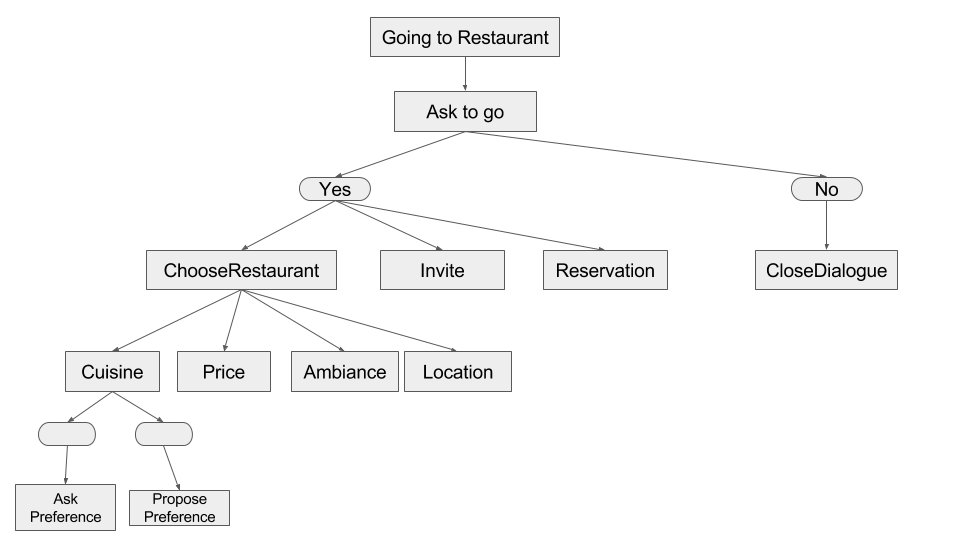
\includegraphics [width=4in]{figs/exemple}}}
	\vskip 8pt
	\defig{ex}{Architecture du modèle de dialogue.}
\end{figure}
L'exemple présenté dans cette section illustre un des premiers dialogues modélisé sous D4g. Le but était de générer un dialogue dont la structure est similaire aux dialogues enregistrés. Par conséquent le but de tâches est de trouver un restaurant. L'arbre de dialogue généré est illustré dans la \fig{ex}. Une partie de l’exécution est présentée ci-dessous.
\begin{verbatim}
    Agent says "Would you to go to dinner with me ?"
  > say
[1] Sure.
[2] No, thanks.
  >> 1     
    User says "Sure."
    Agent says "What kind of food would you like?"
  > say
[1] Japanese
[2] Italian
[3] I don't care !
  >> 3
    User says "I don't care !"
    Agent execute SetUserPreference on I don't care !
    Agent says "Personnally, I'm a huge fan of italian food.
     I know a restaurant called Roseval."
  > say
[1] I heard about that restaurant.
[2] I've never been there.
[3] I hate that restaurant !
[4] I love that restaurant !
  >> 2
    User says "I've never been there."
    Agent says "The problem is that the restaurant is situated
     in a tourestic zone."
  > say
[1] Oh !.
  >> 1
    User says "Oh !."
    Agent says "The best part of this restaurant is the food. 
    All of the dishes are delicious and with huge portions."
  > say
[1] Yes, and their Cabernet Sauvignon is good and not pricey !
[2] That's what I've heard.
[3] It seems good.
\end{verbatim}


\section{Perspectives et travaux futurs}
\label{pers}

Nous avons présenté dans ce rapport les travaux réalisés jusqu'à présent. Les six premiers mois de la thèse ont été consacré à la rédaction d'articles sur le travail réalisé durant le stage de Master. un premier article \cite{ouali2015reparation} publié à la conférence des Jeunes Chercheurs en Intelligence Artificielle (RJCIA 2015), et un second \cite{ouali2015plan} publié à AGI (Artificial General Intelligence). Ensuite, je me suis intéressée à la littérature afin de définir l'aspect social à étudier pour la gestion du dialogue, qui a aboutie sur le choix de l'analyse de relations interpersonnelles dans le dialogue. 

\par Dans le but de concevoir un modèle formel de dialogue social qui prend en compte les relations interpersonnelles, j'ai d'abord réalisé une collecte de données afin d’observer le comportement des interlocuteurs dans le dialogue. L'analyse des dialogues collectés m'a guidé par la suite dans la conception de mon modèle dialogique, d'une part dans le choix de la négociation coopérative sur les préférences dans le dialogue et d'autre part dans la définition des actes de dialogue.  La travail réalisé a aboutie sur la conception d'un modèle de dialogue pour une négociation coopérative qui a été implémenté. 

\par La prochaine étape consiste à tester le modèle de dialogue. Pour se faire, je dois concevoir un protocole de validation qui puisse analyser la perception de l'utilisateur sur sa relation avec l'agent. Cette validation nous orientera sur nos choix pour l'insertion des variables sociales dans les choix des stratégies de dialogue. En parallèle, je prépare un article à soumettre pour la conférence IVA2016. 

\par Le plan des travaux à venir se présente comme suit: D'abord une validation du système actuelle doit être réalisé afin de pouvoir publier un article pour le mois de mai. 
Ensuite, l'arbre de dialogue existant doit être étendu afin qu'il puisse adapter les stratégies de l'agent dynamiquement par rapport à sa perception des relations interpersonnelles (sera réalisé pour l'été 2016). Une étude sur les raisonnements de l'utilisateur durant le dialogue doit être menée (théorie de l'esprit), pour pouvoir valider notre modèle dialogique pour lesquels nous attendons a avoir les résultats pour la fin de l'année 2016.
Enfin la troisième année de thèse sera consacré à la rédaction du manuscrit de thèse et à la publication d'articles.


% ====================================================================					
	\vskip 4pt
	\bibliographystyle{abbrv}
	{\footnotesize
			\bibliography{Library}} % The references (bibliography) information are stored in the file named "library.bib"
	
\end{document}
			
			
